\chapter{Theoretical Foundations}
This chapter presents the theoretical foundations and the current state of research. These serve as the
starting point for the analysis in the expert interviews (see Chapter
\ref{ch:empirical-analysis-of-facilitating-strategies}) and
provide indicators of what to focus on during the subsequent requirements gathering process (see Chapter
\ref{sec:requirements-analysis}).

\section{Remote Meetings (RQ1)}

Some studies define meetings as a goal- or outcome-oriented interaction between two or more
people. \cite[p. 148]{beranekFacilitationGroupSupport1993}
One weakness of this definition is that some meetings would likely fail to meet the
assumption of being goal-oriented.

Kayser \cite{kayserMiningGroupGold1990}, as cited
in \cite{romanoMeetingAnalysisFindings2001}, offers a somewhat humorous definition that nevertheless captures the
ineffectiveness of some meetings: "A meeting is a gathering where people speak up, say nothing, and
then all disagree."

In their literature-based survey of meetings, Romano and Nunamaker derive the following
summarizing definition. A meeting is "a focused interaction of cognitive attention, planned or chance,
where people agree to come together for a common purpose, whether at the same time and the same place, or at
different times in different places.”\cite[p.1]{romanoMeetingAnalysisFindings2001}

This thesis uses the term “meetings” in this board sense of the summarizing definition.

In this thesis, “remote meetings” are defined as meetings that take place synchronously via an online
video conferencing platform.

% ---------------------------------------------------------------------------------------------------------------------
\subsection{Remote Meetings in Modern Work: Trends and challenges}
\label{sec:meetings-in-modern-work}

Although meetings are important for teams to achieve goals, solve problems, and make
decisions, there are many signs that meetings are perceived as ineffective.

One of the most negative evaluations of meetings originates from a study by Atlassian, in which
more than 72\% of meetings were rated as ineffective by participants.
The study identifies therefore problems such as off-topic discussions,
uneven participant engagement, and a lack of structure.
\cite{atlassianWorkplaceWoesMeetings}

Earlier studies on managers' self-assessments of meeting productivity ranged from 33\% to 47\%.
\cite[p. 1]{romanoMeetingAnalysisFindings2001}

In a study by Geimer et al., of the more than 1,000 participants surveyed, fewer than half
considered their typical meetings to be an effective use of time. \cite[p. 2019]{geimerMeetingsWorkPerceived2015} The
most common negative statements were found in the area of “meeting organization.” \cite[p.
2019]{geimerMeetingsWorkPerceived2015}. Examples cited a lack of structure, the absence
of an agenda, or an unclear objective. Generally poor preparation was also mentioned, as well as the fact that
meeting participants had not been provided with all relevant information in advance. \cite[p.
2019f]{geimerMeetingsWorkPerceived2015}

So a clear issue with goal-oriented meetings is the absence or unclear communication of objectives.

An agenda was identified by many respondents (67\%) as a key element for successful meetings in Doodle’s State
of Meetings Report 2019. Only the setting of clear meeting objectives (72\%) was cited even more frequently.
\cite[p. 11]{DoodleStateMeetings2019}

While an agenda can serve as the foundation for such structure, it alone does not guarantee a successful
meeting. Meeting goals are often dynamic and may need to be adjusted as the meeting progresses, due to the associated
uncertainties \cite[chap 4.1]{chenAreWeTrack2025}. Although the agenda can outline a path to achieving the
overall meeting goal \cite[chap 2.1]{scottMentalModelsMeeting2024}, without linked sub-goals, it guarantees
neither the success of the meeting nor a timely conclusion. \cite[chap 4.1]{chenAreWeTrack2025}
Discussions can nevertheless get out of hand if participants do no know what to priorities. \cite[chap
4.1]{chenAreWeTrack2025}

Furthermore, respondents to the study by Geimer et al. mentioned that meetings were often held with
inappropriate participants. People were invited to meetings who had nothing to do with the projects or issues
discussed during the meeting. \cite[p. 2019f]{geimerMeetingsWorkPerceived2015}
Not having the right people in a meeting is one of the main reasons for unproductive meetings.
\cite[p.6]{romanoMeetingAnalysisFindings2001}

Dysfunctional communication—such as complaining, criticizing, and digressing—reduces effectiveness.
\cite[p. 130]{kauffeldMeetingsMatterEffects2012}. It appears that dysfunctional communication has a stronger
impact on the success of a meeting than functional communication. ("bad is stronger than good")
\cite[p. 148]{kauffeldMeetingsMatterEffects2012}

Chen et al. noted, as a secondary finding, that individuals in higher hierarchical positions tended to
intervene more frequently and maintain focus on meeting objectives when a clear list of goals was provided.
Conversely, those in lower hierarchical positions felt less obligated to intervene, even when they observed
deviations from the main topic. \cite[chap 4.3]{chenAreWeTrack2025}
Doodle’s State of Meetings Report 2019 identified a correlation between salary and self-perceived
participation in meetings. Respondents with higher salaries were more likely to describe themselves as active
participants. \cite[p. 6]{DoodleStateMeetings2019}
This may stem from inexperience, hierarchical constraints, group dynamics, or a lack of error culture, where
dissent risks loss of face. Low participation can narrow solution spaces, yield monotonous outcomes, and
reduce meeting effectiveness.

Inclusion in meetings can increase satisfaction, performance, and creativity.
\cite[p.1]{houttiObserveAskIntervene2025}. In addition, this can counteract hidden profiles
(see \autoref{sec:hidden-profiles}).

Most of these insights apply to both remote and in-person meetings. Remote meetings,
however, present additional challenges.

Thus, the main challenges of remote work are technology and communication issues. In addition,
early-morning meetings and the use of video can be sources of stress for meeting participants.
\cite[p.151]{luebstorfDiggingZoomFatigue2023}
It was also observed that multitasking, that is, switching between different activities in a short
period of time, is a critical stressor during video conferences. Multitasking occurred more frequently in
larger meetings with
cameras turned off. \cite[p. 159]{luebstorfDiggingZoomFatigue2023}

Based on the expert interviews with facilitators conducted by Hughes and Roy, it can be concluded that in
in-person meetings, facilitators find it easier to establish a shared “energetic presence,” (including the
perception of participants’ nuances) which is more difficult in a remote setting. One facilitator described
it as if he was almost blind online.
\cite[p.10]{hughesKeeperSynchronousOnline2021}

Taken together, the studies trace the widespread perception of meetings as ineffective to the way the
meeting is conducted: objectives stay unclear or shift without sub-goals that would tell participants
what to prioritize, while unsuitable participants, dysfunctional communication, and hierarchically uneven
participation restrict the knowledge that enters the discussion. For synchronous remote meetings, an
agenda and a stated goal are therefore necessary but not sufficient. Without a structure that can absorb
changing objectives and inclusion that counters status differences, the meeting is unlikely to stay
focused or to close on time.

% ---------------------------------------------------------------------------------------------------------------------
%\subsection{Key challenges: Off-topic discussions, unequal participation, lack of structure}
% \label{sec:key-challenges-in-meetings}
% A clear issue with goal-oriented meetings is the absence or unclear communication of objectives. It seems
% plausible that a significant number of meetings are scheduled without a defined goal or agenda (as
% discussed in section
% \ref{sec:meetings-in-modern-work}).
% A lack of structure in meetings is therefore one of the key challenges.
% While an agenda can serve as the foundation for such structure, it alone does not guarantee a successful
% meeting. Meeting goals are often dynamic and may need to be adjusted as the meeting progresses, due to
% the associated
% uncertainties \cite[chap 4.1]{chenAreWeTrack2025}. Although the agenda can outline a path to achieving the
% overall meeting goal \cite[chap 2.1]{scottMentalModelsMeeting2024}, without linked sub-goals, it guarantees
% neither the success of the meeting nor a timely conclusion. \cite[chap 4.1]{chenAreWeTrack2025}
% Discussions can nevertheless get out of hand if participants do no know what to priorities.
% \cite[chap 4.1]{chenAreWeTrack2025}
% An agenda was identified by many respondents (67\%) as a key element for successful meetings in Doodle’s State
% of Meetings Report 2019. Only the setting of clear meeting objectives (72\%) was cited even more frequently.
% \cite[p. 11]{DoodleStateMeetings2019}

% Based on this, the following summary challenge statement was derived:

% \begin{quote}
%   \textbf{Challenge 1: Clear goal-setting and structure.}
%   \label{chal:clear-goals-and-structure}
%   Goal-oriented meetings frequently lack clearly communicated objectives and a reliable structure, so that
%   discussions lose focus and the meeting neither succeeds nor concludes on time.
% \end{quote}

% Chen et al. noted, as a secondary finding, that individuals in higher hierarchical positions tended to
% intervene more frequently and maintain focus on meeting objectives when a clear list of goals was provided.
% Conversely, those in lower hierarchical positions felt less obligated to intervene, even when they observed
% deviations from the main topic. \cite{chenAreWeTrack2025}
% Doodle’s Stat of Meetings Report 2019 identified a correlation between salary and self-perceived
% participation in meetings. Respondents with higher salaries were more likely to describe themselves as active
% participants. \cite[p. 6]{DoodleStateMeetings2019}
% This may stem from inexperience, hierarchical constraints, group dynamics, or a lack of error culture, where
% dissent risks loss of face. Low participation can narrow solution spaces, yield monotonous outcomes, and
% reduce meeting effectiveness.

% Dysfunctional communication—such as complaining, criticizing, and digressing—reduces effectiveness.
% \cite[130]{kauffeldMeetingsMatterEffects2012}

% -> Unausgeglichen / geringe participation
% -> Unvorhergesehen veränderungen im Meeting (flasch Annahmen, meetingziel ändert sich)
% -> technische Probleme: Instablie internetverbindungen, Störungen etc. (nicht im scope dieser arbeit aber
% dennoch relevant)

% Graph der zeigt das sich diese challanges alle gegenseitig beiflussen könnnen. (z.B. wenn nicht nicht alle
%   ansichten geührt wurde, kann es später dazu kommen das wenn man eigentlich eien entscheidung treffen möchte
% (convergent thinking) wieder zurück in divergent htink fällt, was zu zirkuläeren diskussionen führen kann.)

% Umgekert, kann ein zulanges verweilen in der coonvergnen zone dazuführen, dass kein entshciedung getroffen
% wird und kein fortschirtt wahrgenommen wird.

% temkultur und hierarchie beinfluss ebenfalls die offen tielnehmer ideen teilen und wer welche ideen wie bewertet.

% Aus den experten Interviews mit Facilitatoren von Hughes und Roy \cite{hughesKeeperSynchronousOnline2021}
% lässt sich ableiten, dass in physischen Treffen Facilitatoren leichter eine gemeinseme "energetische Präsenz"
% aufbauen udn Momente der Spannung im Raum leicher halten können. aus diesen würden oft die eigentlichen
% "Aha-Momente" und kreativen Druchbrüche entstehen. Im
% remote Kontext sei es schwer diese Spannung aufrechtzuerhalten, da man sich physich distanziert fühle und oft
% "bild" für die feinen emotionalen Schwingungen der anderen sei. \cite["5.5 Unstructured Expert
% Interviews"]{hughesKeeperSynchronousOnline2021}

\section{Facilitation and Convergent Group Decision-Making (RQ1)}
\label{sec:facilitation-and-group-decisions}

% % ---------------------------------------------------------------------------------------------------------------------
% \subsection{The facilitator role}
% The book *Facilitation Fundamentals* by AJ\&Smart \cite{aj&smartFacilitationFundamentalsWorkbook}, one of the
% leading companies in the field of facilitation and facilitator training, introduces the 4C framework. This framework
% classifies methods that can be used in meetings or workshops into four key categories:

% \begin{itemize}
%   \item Collect: Suitable for systematically gathering and visualizing information within a team.
%   \item Choose: Narrows down a large number of ideas or content to a few selected elements.
%   \item Create: Uses design thinking methods to develop new approaches to solutions.
%   \item Commit: Ensures the team’s binding agreement on the decisions made and the results achieved.
% \end{itemize}

% As outlined in the chapter “Convergent and Divergent Thinking,” a clear distinction between the divergent and
% convergent phases is crucial. The 4C framework, which many facilitators rely on, enables
% the implementation of these best practices.

% \section{Convergent Decision-Making in Groups (RQ1)}

% ---------------------------------------------------------------------------------------------------------------------
\subsection{Group Support Systems and collaboration tools}
\label{sec:gss-collaboration-tools}

Research on group support systems (GSS) began in the 1980s in response to the constant challenges posed by
increasingly complex problems that often had to be solved in groups or teams within organizations.
\cite[p. 628]{ackermannGroupSupportSystems2021}

According to Ackerman, the early days of this field of research were marked by significant fragmentation.
Various research teams worked independently of one another and without coordination on overlapping topics.
\cite[p.628]{ackermannGroupSupportSystems2021}

As a result, there was no standardized approach, and different terms for
the same field of research became established, such as “Meeting Support Systems,” (MSS) “Computer-Supported Cooperative
Work Systems,” (CSCW) “Group Support Systems,” (GSS) or “Group Decision Support Systems” (GDSS).
\cite[p.628f]{ackermannGroupSupportSystems2021}

In some cases, the term “electronic meeting system” (EMS) is also used. This term was coined by
Dennis et al. when they attempted to bring the two research areas, GDSS and CSCW under a single
definition. \cite[p. 592]{dennisInformationTechnologySupport1988}

According to Dennis et al., GDSSs have focused more strongly on tasks
such as decision-making, planning, and problem-solving, while CSCWs are geared more toward communication
needs. However, the authors themselves note that there are only subtle differences
between these areas and predict that the various system classes will eventually be merged into a single class
. \cite[p. 592]{dennisInformationTechnologySupport1988}

The terms GSS, GDSS, and EMS can therefore now be considered synonymous. \cite{ElectronicMeetingSystem2025}

The overarching goal of the various lines of research is to collectively optimize meetings in terms of
both the quality of their outcomes and the structure of their processes.
\cite[p.629]{ackermannGroupSupportSystems2021}

Computer-aided tools are often used for this purpose. Huber defined it as follows
\cite[p. 195]{huberIssuesDesignGroup1984a}:

\begin{quote}
  "GDSS consists of a set of software, hardware, and language components and procedures that support a group
  of people engaged in a decision-related meeting."
\end{quote}

GSSs are thus a combination of methodological structures and processes that are documented in a way that
makes them usable by groups,
as well as technical tools designed to make the use of these methods practical during
meetings.

Group Support Systems (GSS) can vary greatly in terms of their complexity and functionality

Some systems allow participants to enter text contributions simultaneously and anonymously in order to
conduct electronic
brainstorming, criteria analyses, or prioritization votes. One example of this is
GroupSystems (later known as ThinkTank, presumably based on Plexsys)
\cite[p.634]{ackermannGroupSupportSystems2021}.

Plexsy is a framework presented by Dennis et al. that made various facilitation methods available for groups using
supporting IT systems. It includes, for example, methods such as electronic brainstorming, voting
procedures (prioritizing, Likert scales, multiple-choice questions, etc.), and several other approaches. \cite[p.
606f.] {dennisInformationTechnologySupport1988}
Depending on the phase of the meeting, the group can select an appropriate method and switch between them
. \cite[p. 607]{dennisInformationTechnologySupport1988}

Group Explorer, which has evolved from its single-user predecessors COPE and Decision Explorer into today’s web platform
"Strategyfinder"\cite{InteractiveDecisionMakingPartner}, is a visual group support system that models complex
group problems as interactive cause-and-effect networks (Cause Maps). In these maps, the causal relationships
(in the sense of “A leads to B”) expressed by the participants (in the sense of “A leads to B”) are
graphically linked together. The goal is to make complex relationships understandable and visual in order to
facilitate joint decision-making. \cite[p. 636f]{ackermannGroupSupportSystems2021}

With the further development of GSS, the Thinklets Framework has become established as a way to encapsulate formalized
facilitation techniques and proven procedures used by facilitators, in order to generate predictable and
repeatable behavioral patterns in collaborative groups. They consist of small, standardized tools
and scripts designed to enable groups to accomplish group tasks. \cite[p.
635]{ackermannGroupSupportSystems2021}

Modern tools such as Miro, Conceptboard, or Figma Jam, which can be classified as digital whiteboard solutions or CSCW,
draw on some of these original methods
(such as asynchronous information gathering, private information sharing, and voting (anonymous or
non-anonymous)) and combine them with the capabilities
offered by modern technologies that enable distributed collaboration.

Integrated AI-based features enhance these tools with smart functions such as the automatic grouping of ideas
into topic clusters by AI
or the enrichment of ideas through AI-generated suggestions
(see \autoref{sec:existing-meeting-ai-tools}).

In addition, there are various modern collections of exercises, methods, and tools—including instructions for
carrying them out (similar to the Thinklets concept), as well as guidance on what to look out for, which are suitable
for various group situations and challenges in meetings, such as:
\begin{itemize}
  \item Liberating Structures: A collection of methods, tools and templatesfor facilitation.
    \cite{LiberatingStructuresInnovation2024}
  \item 9 Spaces: A collection of methods, tools and templates for facilitation. \cite{9SpacesEntwickle}
  \item SessionLab Library: SessionLab is a tool for creating workshop agendas. There is a
    community-maintained library where many methods are shared. \cite{sessionlabsDesignFasterAI2025}
\end{itemize}

In GSS research, there were approaches that assumed that GSS, due to the intuitly aimed
interface design, could be operated independently by group members.
However, as system and task complexity increased, it proved difficult in practice to simultaneously
participate substantively in the discourse, operate the technical GSS software, and moderate the group process. \cite[p.
631]{ackermannGroupSupportSystems2021}

As a result, an additional, somewhat rigid role structure emerged at that time: In addition to the
facilitator, who focused on content and social dynamics,
a so-called “chauffeur”, decribe by Whiteley and Garcia was as the “technical support person,” responsible
for the purely technical
control of the GSS. \cite[p. 31]{whiteleyFacilitatorChauffeurGSS1996}

This historical necessity of providing two highly specialized roles—even though the role of the
“Chofferus” has become obsolete today—underscores just how complex it
is to conduct meetings effectively, even with support systems.

% ---------------------------------------------------------------------------------------------------------------------
\subsection{The facilitator role}
\label{sec:facilitation}

Even in the early days of GSS (Group Support Systems) research, Beranek et al. pointed out that GSS
alone likely cannot guarantee the effectiveness of a session. Rather, success
depends largely on how these systems are used. \cite[p. 147] {beranekFacilitationGroupSupport1993}
In this context, the quality of the group session would depend largely on the facilitator.
\cite[p.146]{beranekFacilitationGroupSupport1993}

In the German-speaking context, the term “facilitator” is sometimes mistakenly translated as “moderator.” However, this
equivalence is inadequate, as the roles have different focuses: While a
moderator is primarily responsible for managing a meeting, a facilitator’s role is aimed at
supporting the group in terms of both process and content. Although the role of the facilitator includes
elements of moderation,
it goes beyond that

According to Haney, researchers in the 1990s agreed that facilitation is a combination of
“(1)managing relationships between people, tasks and technology, (2) structuring tasks, and (3) contributing to
the effective accomplishment of the meeting outcomes.” \cite[p. 73]{hayneFacilitatorsPerspectiveMeetings}

In his book "The Skilled Facilitator", regarded as a standard work in the field, organizational
psychologist Roger Schwarz defines the term “Facilitator” as follows:
(\cite{schwarzSkilledFacilitatorComprehensive2016} as cited in
\cite{parsonsdialogueWhatMakesGood} \& \cite[p.9]{aj&smartFacilitationFundamentalsWorkbook}):

\begin{quote}
  "Group facilitation is a process in which a person who is acceptable to all members of a group,
  substantively neutral, and has no decision making authority, intervenes to help a group improve the way it
  identifies and solves problems, and makes decisions, in order to increase the group’s effectiveness."
\end{quote}

Whiteley and Garcia attribute a number of key functions to a facilitator working in conjunction with a GSS.
These include, process and agenda management, in which the facilitator guides the group through the
problem-solving process and the agenda, but must adapt these flexibly and in real time when new problems arise. \cite[p.
36]{whiteleyFacilitatorChauffeurGSS1996} \cite[p. 31]{whiteleyFacilitatorChauffeurGSS1996}
In addition, the facilitator is responsible for mood and relationship management (mood making)
\cite[p.33]{whiteleyFacilitatorChauffeurGSS1996} , which includes
assessing when the group’s mood needs to be lifted
or lowered, and when to intervene, confront, calm, or reconcile.
\cite[p.31]{whiteleyFacilitatorChauffeurGSS1996}
Furthermore, the facilitator is responsible for creating a trusting work environment by
setting guidelines and establishing a high-trust environment.
\cite[p.31]{whiteleyFacilitatorChauffeurGSS1996}
The facilitator interprets and perceives symbolic signals, uncovers myths and hidden interests, and
refocuses the discussion on the actual core issues through framing.
\cite[p.32]{whiteleyFacilitatorChauffeurGSS1996}
In addition, the facilitator supports interest-based negotiations,
consensus building, and the promotion of effective interpersonal behaviors to enable teamwork.
\cite[p.34]{whiteleyFacilitatorChauffeurGSS1996}

In summary, according to Whiteley and Garcia, a facilitator needs skills in the following areas:
problem-solving, decision-making, discrimination, reflection, imaging, intuiting, emotional, and being
skills. These range from structured problem-solving and evaluation to causal, systemic, and
lateral thinking, as well as visualization and pattern recognition. In addition, there are emotional skills such as
humor and self-esteem, as well as “being” skills, which are characterized by resonance, balance, and autonomy
within the group. \cite[p.34]{whiteleyFacilitatorChauffeurGSS1996}

% ---------------------------------------------------------------------------------------------------------------------
\subsection{Divergent and Convergent Thinking in Meetings}
\label{sec:divergent-convergent}
Divergent thinking is the process of generating new ideas and concepts [TODO: QUELLE]. Convergent thinking is
the process of evaluating and selecting the best ideas from a set of options. [TODO: QUELLE]

According to Anne Manning, generating new ideas and evaluating them are two fundamentally different
processes. However, she says that in meetings, people often try to carry out both steps at the same time.
\cite[min 02:30]{professional&executivedevelopment-harvarddceConvergentVsDivergent2024}
Immediately evaluating and weighing an idea hinders the creative process of generating ideas.

A predominance of divergent thinking without sufficient integration of convergent thought processes can lead
to unreflective and excessive modifications. \cite{cropleyPraiseConvergentThinking2006} Corply
\cite{cropleyPraiseConvergentThinking2006} further argues that both a lack and an excess of
convergent or divergent thinking have adverse effects on creativity.

In the context of facilitation, the terms "Convergence Zone / Phase" and "Divergence Zone / Phase" are
widely recognized. A recurring framework in this domain is the group process map, developed by facilitator
Sam Kaner, commonly referred to as "Diamond of Participatory Decision-Making" or "Kaner’s Diamond".
\cite{kanerFacilitatorsGuideParticipatory2014}
Kaner’s Diamond model describes typical phases that groups go through in the decision-making process. The left
side represents the Divergent Zone, where diverse perspectives are expressed and disagreements are explored.
The right side embodies the Convergent Zone, where opinions align and the process moves toward closure. At
the center of the Diamond lies the "Groan Zone", a transitional phase where the tension between divergence
and convergence often manifests.

% ---------------------------------------------------------------------------------------------------------------------
\subsection{Biases in information exchange (Hidden profiles)}
\label{sec:hidden-profiles}

Diese Arbeit geht von der Hypothese aus, dass ein proaktives Meeting-Supporsystem insbesondere dort
eine Lücke schließen kann, wo die Gruppe ihre eigene Ineffizienz nicht erkennt. Ein interaktives
System setzt voraus, dass Teilnehmende ein Problem bemerken und um Unterstützung bitten. Genau das
entfällt, wenn der Prozess subjektiv reibungslos wirkt, obwohl er systematisch verzerrt ist.

Typischerweise liegt diese Unbewusstheit bei Biases vor, etwa Confirmation Bias, Groupthink,
Authority Bias, Halo-Effekt, Anchoring oder Status-Quo-Bias, um nur ein paar zu nennen.

Nach den Experten interviews und bei beim desing des system wurde sich dafür entschiende sich auf Hidden Profiles zu
fokussieren.

In Meetings verfügen Teilnehmende
typischerweise über unterschiedliche Informationen. Einen Teil kennen alle (geteilte Informationen),
einen anderen Teil nur einzelne Personen (ungeteilte/private Informationen).

Dieses Problem wird in der Literatur als Hidden-Profile-Paradigma beschreiben.

Dieses Problem wird in der Literatur als Hidden-Profile-Paradigma beschreiben. In Meetings verfügen Teilnehmende
typischerweise über unterschiedliche Informationen. Einen Teil kennen alle (geteilte Informationen),
einen anderen Teil nur einzelne Personen (ungeteilte/private Informationen). Ein Hidden Profile liegt vor,
wenn die bessere Lösung nur sichtbar wird, sobald die ungeteilten Informationen zusammengeführt
werden. Gruppen diskutieren jedoch vorwiegend geteilte Informationen und ungeteilte informationen kommen zu
krz oder werden nicht erwähnt.
\cite{stasserExpertRolesInformation1995,arkesInformationExchangeGroup2009,bakerEnhancingGroupDecision2010}.

Confirmation Bias und Groupthink verstärken diesen blinden Fleck, weil einzigartige Informationen den bestehenden
Konsens stören \cite{bakerEnhancingGroupDecision2010,schulz-hardtGroupDecisionMaking2006}.
Ohne externe Intervention bleibt die Ineffizienz unbemerkt.

Laut Verhein-Jarren et al. ist Voraussetzung für eine gute Kommunikation das Erkennen des eigenen
Persönlichkeitsstils sowie das Wissen darum, dass es verschiedene Bezugswelten gibt, in denen sich die
Beteiligten während des Gesprächs bewegen. Menschen neigen dazu, andere unbewusst nach eigenen Mustern zu
interpretieren. Laut Verhein-Jarren et al. sei ein Durchbrechen dieses Automatismus der Wahrnehmung
notwendig, um einen geteilten Bezugsrahmen zu schaffen. \cite[p.
9]{verhein-jarrenGespraechsfuehrungTechnischenBerufen2018}

Innerhlab des bleichen bezugsrahmen, kann es dann allerdgins druch aus auch zu meindugnsverscheidnheiten
kommen, was nicht unbedingt schlecht ist. Schulz-Hardt et al. (2006) zeigen empirisch, dass
Meinungsverschiedenheiten (Dissent) die Diskussionsintensität massiv erhöhen und die Lösungsrate des Hidden
Profiles drastisch steigern. \cite{schulz-hardtGroupDecisionMaking2006}

Nicht alle diese Verzerrungen greifen jedoch am selben Punkt an.
Authority Bias oder Halo-Effekt betreffen vor allem, wessen Beitrag
oder welcher Gesamteindruck übergewichtet wird. Confirmation Bias und Groupthink betreffen
dagegen, welche Informationen überhaupt geteilt und diskutiert werden.

Für die konvergente Phase wird daher angenommen, dass zunächst vor allem der Informationsaustausch
als grundlage entscheidungsrelevant ist.

%%%%%%%%%%%%%%%%

Geteilte vs. Ungeteilte Informationen: Das Hidden Profil

Ein typisches Experiment, um Entscheidungsprozesse in Gruppen zu untersuchen sieht folgendermaßen aus: Ein
Team hat die Aufgabe aus unterschiedlichen BewerberInnen den Besten oder die Beste auszuwählen. Dazu erhält
jedes Team-Mitglied Informationen über die einzelnen BewerberInnen. Einen Teil der Information erhalten alle
Teammitglieder. Diese Informationen sind also im Team geteilte Informationen. Einen anderen Teil der
Informationen erhält jeweils nur ein Team-Mitglied. Diese Informationen sind also ungeteilt. Die Aufgabe ist
nun so konstruiert, dass sich das Team nur dann für den richtigen Bewerber entscheiden kann, wenn alle
Informationen – geteilte und ungeteilte – berücksichtigt werden. Werden lediglich die geteilten Informationen
berücksichtigt, trifft das Team eine falsche Entscheidung.

Eine Vielzahl von Studien mit dieser oder ähnlichen Aufgaben zeigt, dass Teams meist nicht in der Lage sind,
ein solches Hidden-Profile zu lösen: Geteilte Informationen werden ausgetauscht und diskutiert, ungeteilte
Informationen fallen unter den Tisch.
Erklärungen für das Phänomen Hidden Profil

Es gibt unterschiedliche Erklärungen dafür, warum in Gruppendiskussionen eher über geteilte Informationen
gesprochen wird:

Wahrscheinlichkeit: Mehr Personen verfügen über die gleiche geteilte Information. Deshalb ist die
Wahrscheinlichkeit höher, das geteilte Informationen in der Gruppe diskutiert werden, im Vergleich zu
Informationen, über die nur eine einzelne Person verfügt (ungeteilte Informationen).
Selbstwerterhaltung: Menschen achten darauf, ein positives Selbstwertgefühl zu erhalten. Wird eine geteilte
Information der Gruppe mitgeteilt, werden andere Personen in der Gruppe dieser Information zustimmen, bei
ungeteilten Informationen steigt die Gefahr, kritisiert zu werden. Das gefährdet ein positives
Selbstwertgefühl, weshalb eher ohnehin schon geteilte Informationen der Gruppe mitgeteilt werden.
Group Think: Jedes Gruppenmitglied hat das Bedürfnis, sich der Meinung der Gruppe anzuschließen. Die Gruppe
als Ganzes strebt nach Konsens. Das kann dazu führen, dass kritische oder widersprüchliche Informationen
nicht ausreichend berücksichtigt werden.

Lösungsstrategien für das Hidden Profil

Die Forschung zu Hidden-Profiles basiert auf eher künstlichen Gruppensituationen. Dennoch lassen sich aus den
Ergebnissen Strategien ableiten, Gruppenentscheidungen zu verbessen.

Effekt kennen: Wer die Anfälligkeit von Gruppen kennt, ungeteilte Informationen zu vernachlässigen, kann
gezielt gegensteuern. Eine Möglichkeit ist z. B. nachzufragen, ob alle Informationen berücksichtigt wurden,
oder ob es Informationen gibt, die nicht ins Bild passen.
Expertise transparent machen: In einer heterogenen Gruppe hilft es, die unterschiedlichen Fach- und
Wissensgebiete der einzelnen Mitglieder transparent zu machen. So wird klar, dass unterschiedliches Wissen
und unterschiedliche Meinungen zu erwarten sind.
Technische Unterstützung: Technische Werkzeuge, die Informationen visualisieren oder strukturieren, helfen
insbesondere bei komplexen Entscheidungen, alle Informationen zu berücksichtigen.
Erst suchen, dann bewerten: Eine weitere Strategie ist es, das Sammeln und das Bewerten von Informationen als
zwei Prozesse voneinander zu trennen. So wird verhindert, dass Informationen, die wichtig sein könnten,
direkt abgewertet werden.
Hierarchien vermeiden: Oft teilen insbesondere Mitglieder mit niedrigem Status ihr ungeteiltes Wissen nicht,
wohingegen geteiltes Wissen, dass Mitglieder mit hohem Status eingebracht haben, detailliert diskutiert wird.
Eine Lösungsstrategie ist deshalb, dass sich die Gruppenleitung oder Mitglieder mit hohem Status zunächst mit
einer eigenen Bewertung zurückhalten.

%Literaturhinweis: Stasser, G., \& Titus, W. (1985). Pooling of unshared information in group decision making:
%Biased information sampling during discussion. Journal of Personality and Social Psychology, 48, 1467–1478.

%Literaturnachweis: Stasser, G., \& Titus, W. (1985). Pooling of unshared information in group decision making:
%Biased information sampling during discussion. Journal of Personality and Social Psychology, 48, 1467–1478.

%Zitieren als: Moskaliuk, J. (2013). Warum Gruppen falsch entscheiden. wissens.blitz (95).
%https://wissensdialoge.de/hidden_profile

\section{AI in Meeting Support Systems (RQ2)}

In addition to the fundamentals of Group Support Systems (GSS) outlined in
\autoref{sec:gss-collaboration-tools}, modern approaches
specifically designed for meeting support systems can be identified, some of which are supplemented by
functions that are more or less supported by AI. This chapter analyzes these systems to identify potential
gaps and to serve as a source of inspiration for the development of the prototype.

% ---------------------------------------------------------------------------------------------------------------------
\subsection{Overview of existing Meeting AI Tools}
\label{sec:existing-meeting-ai-tools}
There is a wide variety of AI-based tools that provide support for meetings. Most of these tools focus on
transcribing meeting content. Well-known examples include fireflies.ai \cite{Firefliesai1AI}, Otter.ai
\cite{otteraiOtterMeetingAgent}, and Jamie \cite{jamieaiJamieYourPersonal}.
AI transcription features are also integrated into established meeting platforms such as Google Meet
\cite{workspaceGoogleMeetTelefon}, Zoom \cite{zoomKINotizentoolIhrKIMeetingAssistent},
and Microsoft Teams. \cite{microsoftVideokonferenzenBesprechungenAnrufe}
More advanced features include the automatic extraction of action items. Depending on the tool, these
features are available in real time or only after the meeting has ended.
Microsoft Teams specifically offers a feature called “Facilitator,” \cite{microsoftSetFacilitatorMicrosoft}
which provides additional capabilities beyond the features already mentioned (transcription, identification
of action items): For example, it can edit the agenda if instructed to do so by a user with the appropriate
permissions. It also displays a timeline to track topics and the flow of the meeting, and sends reminders to
manage time. (Once halfway through the meeting and again shortly before it ends.) These interactions take
place via the integrated chat.
Google Meet, for example, also offers a live speech translation feature. \cite{googleLearnSpeechTranslation}

Nevertheless, contemporary meeting platforms remain primarily technical infrastructures for conducting
meetings. Their design does not systematically account for the professional knowledge, needs, and
methodological repertoire of facilitators \cite{hughesKeeperSynchronousOnline2021}, nor are they conceived to
support the range of tools, methods, practices, and techniques on which facilitation typically relies.

There are also platforms specialized for facilitation needs, such as Stormz \cite{GetStartedStormz}, offer AI
support across different phases of a meeting, including brainstorming.
\cite{aitinkerersclubStormzAIFeature2023}

Platforms such as SessionLabs curate methods from the facilitation community and, with the help of an AI
assistant, make it possible to find suitable methods and generate an agenda tailored to the meeting's
objectives.\cite{sessionlabsDesignFasterAI2025}

% ---------------------------------------------------------------------------------------------------------------------
\subsection{Related Research Approaches to AI-Supported Meeting-Systems}
\label{sec:research-approaches-to-ai-supported-meeting-systems}
Several works in the literature pursue a comparable approach or related research questions . Among them, two
papers proved particularly relevant to this thesis. Their key findings are summarized below to clarify how
they inform the subsequent work.

\textbf{Are We On Track?}

In an empirical study involving 15 knowledge workers, Chen et al. examined how AI can
support goal orientation and intentionality in meetings through passive visual cues and active, inquiry-based
reflection prompts. \cite[p. 1]{chenAreWeTrack2025}
To increase ecological validity, the authors used past meeting recordings provided by the study participants
and applied a video-stimulated method in which the participants
rewatched the same meeting situation, with the addition that it now included AI interventions.
They evaluated counter-scenarios with simulated AI interventions. \cite[p. 4]{chenAreWeTrack2025}
Technically, the prototypes developed were based primarily on GPT-4, which processed transcripts in simulated
real time to passively visualize topic progression using D3.js or actively display context-related reflection questions.
\cite[p. 6]{chenAreWeTrack2025}
The results show that passive visualizations maintain the flow of conversation and promote individual
understanding, whereas active AI questions, while triggering immediate adjustments, carry the risk of
disruptions to the discourse. \cite[p. 2]{chenAreWeTrack2025} However, due to the passive designs,
particularly in the visualization system,it was found that participants overlooked or ignored them. \cite[p.
2]{chenAreWeTrack2025}
Based on the participants’ responses, the authors conclude that it should be possible to
dynamically adjust the intensity of the intervention to the subjective need for support in order to ensure a
balance between
democratic participation, efficiency, and user control. \cite[p. 13]{chenAreWeTrack2025}

One limitation of this study is that the system was not tested in the context of a live meeting
.

\textbf{Observe, Ask Intervene: designing AI Agents for More Inclusive Meetings}

In the study by Houtti et al., the authors examined the design of an AI agent as a so-called “virtual
co-host” to specifically promote inclusion and equal participation in video conferences.\cite
{houttiObserveAskIntervene2025}
First, ideation sessions were conducted in which participants were asked to design a virtual co-host
that could intervene to balance out inequalities in participation. \cite[p.
6]{houttiObserveAskIntervene2025}

This concept was then evaluated in an exploratory laboratory study involving 68 participants in 12
groups, using a structured decision-making task (“Lost at Sea”) on Discord, followed by questionnaires
on meeting quality and 18 qualitative interviews. \cite[p. 14]{houttiObserveAskIntervene2025}

Technically, the prototype was implemented as a Discord bot in Python (`Discord.py`), which used Selenium and
custom JavaScript to track the cumulative speaking times of all participants in the browser interface in
real time. The bot communicated exclusively via private direct messages, generated
individual bar charts showing speaking time, and always waited for a speaking pause of
at least five seconds before sending messages to avoid interrupting the conversation.
\cite[p.6]{houttiObserveAskIntervene2025}

A tendency was observed to design the AI facilitator in a rather reactive manner. The participants wanted to retain a
certain degree of control over the co-host. \cite[p.6]{houttiObserveAskIntervene2025} Nevertheless, the
authors concluded that this is not always feasible, because they suspected that a system that
must always be triggered might remain unused.
Based on this, the authors derive a framework they call “Observe, Ask, Intervene.”
The AI agent continuously observes the meeting but asks a human participant for permission before intervening.
Nearly all interviewees stated that they would prefer to be asked before an intervention affecting them takes
place. \cite[p.15] {houttiObserveAskIntervene2025}

Specifically, this worked as follows: After certain thresholds for distributed speaking time were reached,
the bot sent a private direct message with questions to people who had a low level of participation. Only
after the person responded accordingly did the agent send the speaking time charts.

Although private feedback was perceived as socially acceptable\cite[p.17]{houttiObserveAskIntervene2025},
the bot did not exert sufficient social or normative pressure, which is why facilitators or dominant speakers
largely ignored or rationalized the AI’s critical feedback.
\cite[p.18]{houttiObserveAskIntervene2025}

It should also be noted that the system is a rule-based prototype that does not utilize a generative LLM pipeline.

% ---------------------------------------------------------------------------------------------------------------------
\subsection{Proactive AI-Interactions: From Turn-Taking to intrinsic Motivation with the Inner Thoughts Framework}
\label{sec:proactive-ai-interactions}

So an AI-System can proactivly interact and therefor reduese the need for explicit prompts by the meeting participants
it should be able to proactively recognize when it is its turn in an interaction sequence.

In dyadic human-AIinteractions, pauses or so-called “stop words” are often
used for this purpose to identify a change in speaker. In multi-party scenarios (e.g., group conversations),
however, this becomes significantly more complex and leads to the “multi-party turn-taking
problem”. \cite{sacksSimplestSystematicsOrganization1974}

Some approaches model the problem as a machine learning task by attempting to predict the next speaker based
on previous speaker changes.
\cite{bayserLearningMultiPartyTurnTaking2019}
Bayer et al. employ traditional algorithms such as Maximum Likelihood Estimation (MLE) and Support Vector
Machines (SVMs), as well as deep learning architectures including Convolutional Neural Networks (CNN) and
Long Short-Term Memory (LSTM) networks.

With these approaches, however, it remains unclear why an agent should interact at a specific point in time.
Due to the design of the ML algorithms, the timing of the interaction is decoupled from its cause or is only
implicitly included in the model, but cannot be explicitly explained.

A naive approach to turn-taking prediction would be to prompt an LLM to ask who is next.

Liu et al. investigated various language models (including GPT-3.5, GPT-4o, and fine-tuned variants) with
regard to their ability to predict the next speaker (next-speaker prediction). They showed that these
approaches work well when speaker identification (turn allocation) is explicit.
\cite[p.4]{liuProactiveConversationalAgents2025}

This makes sense, since the current speaker explicitly assigns the next turn to a specific person, and the
conversational context thus contains clear semantic cues, such as direct mentions of names—that an LLM should
be able to process well.

However, in self-selection scenarios, where a participant chose themselves as the next speaker without being
asked to do so, all models performed no better than chance.
\cite[p.4]{liuProactiveConversationalAgents2025}

The authors conclude from this that the conversational context alone is insufficient for self-selection*
scenarios, and that hidden, internal factors (such as interest, relevance, or motivation to engage) play a
decisive role. \cite[p.4]{liuProactiveConversationalAgents2025} Based on a
thinking-aloud study with 24 participants, they concluded that people are driven by intrinsic motivation to
voice their thoughts. \cite[p.2]{liuProactiveConversationalAgents2025}

Building on this, they modeled a framework for chatbots that they call “Inner Thoughts.” An LLM-based agent
continuously generates internal thoughts in parallel with the conversation and evaluates them based on a
defined heuristic (a fixed prompt in the LLM call). If the intrinsic motivation (i.e., the evaluation of a
thought) exceeds a configurable threshold, the agent decides whether to participate, taking into account the
turn-taking type. \cite{liuProactiveConversationalAgents2025}

In chat evaluations, this system achieved significantly higher performance in self-selection scenarios
than conventional baselines, and human evaluators perceived the conversations as significantly
more natural, intelligent, and coherent. \cite[p.2]{liuProactiveConversationalAgents2025}

\section{LLM-based AI-Systems and Agents in General (RQ2)}
\label{sec:ai-agents}

The previous chapters examined remote meetings, facilitation, and existing GSS primarily from an application
perspective. In the case of the last, technical approaches were also described. To address RQ2,
typical patterns to LLM-based AI systems are also relevant, as well as the possibility of testing these
assumptions. However, this chapter does not claim to be exhaustive but serves primarily to clarify what the
author has focused on.

% ---------------------------------------------------------------------------------------------------------------------
\subsection{Agentic Systems vs. Programmatic Automation / Workflows}
\label{sec:agentic-systems-vs-programmatic-automation-workflows}

Huang explains that it is difficult to provide a correct and complete definition of the term “AI agent”
because our understanding of it and the technologies behind it are changing rapidly. \cite[p.
2]{huangAgenticAITheories2025}

In addition, there is a subjective impression that the term “AI agent” is used excessively and inconsistently
in the literature, which leads to a diffuse understanding of the concept. To narrow down the definition of
the term, this thesis attempts to approach the concept by distinguishing it from programmatic automation methods.

In this thesis, “programmatic process automation” refers to the rule-based automation of
workflows, in which defined conditions and structured decision-making logic are used to execute processes efficiently,
reliably, and reproducibly.

While traditional software executes predefined instructions, “AI agents possess the capacity to initiate
actions, make decisions, and pursue goals without constant human intervention” \cite[p. 2]{huangAgenticAITheories2025}

Thus, AI agents have a higher degree of autonomy in this context.

Anthropic uses the following definition for LLM-based workflows and agents:

\begin{quote}
  "Workflows are systems where LLMs and tools are orchestrated through predefined code paths.
  Agents, on the other hand, are systems where LLMs dynamically direct their own processes and tool usage,
  maintaining control over how they accomplish tasks." \cite{anthropicBuildingEffectiveAI}
\end{quote}

Existing papers, such as the study by Houtti et al. or by Liu et al.
\cite{liuProactiveConversationalAgents2025}, also refer to an AI agent, for example, although it is
questionable whether these can be classified as AI agents according to Antroplic’s definition or whether they
are rather LLM-based workflows.
The system developed by Houtti et al. does not use any LLMs. The authors themselves state that they used a
rule-based prototype system to perform better testing. \cite{houttiObserveAskIntervene2025} Nevertheless,
they refer to it as an AI agent.

For the purposes of this thesis, it should therefore suffice for now to provide a rough classification of
whether the developed system is more agent-based or workflow-based. In this thesis, therefore mostly uses the
general term “AI system” for certain conclusions or system descriptions. When other systems are cited and the
authors use the term “AI agent,” this term has been adopted.

A description of the actual system can be found in the section on system architecture.

% ---------------------------------------------------------------------------------------------------------------------
\subsection{Prompt Engineering and Context Engineering}
\label{sec:context-engineering}

In general, context engineering refers to the design, organization, and management of context-sensitive information,
so that machines act in accordance with human intent. \cite[p. 3]{huaContextEngineering202025}

Although context engineering already played a role in early human-computer interaction frameworks
\cite[p. 1]{huaContextEngineering202025}, research has recently placed greater emphasis on this field due to
the growing challenges in
human-agent interaction (HAI).

In their meta-study \cite{meiSurveyContextEngineering2025}, Mei et al. (2025) analyzed over 1,400 research
papers on the topic of context engineering for LLMs. According to the authors, LLMs have evolved from simple
systems that merely follow instructions (so-called prompt engineering) into central inference modules. In the
process, the design and management of information content has developed into a discipline in its own right
(context engineering) \cite{meiSurveyContextEngineering2025}

For LLM-based systems, context engineering can be defined as follows::

\begin{quote}
  "Context engineering is the practice of deliberately structuring and optimizing the information passed to an
  LLM or Agent to produce more accurate and relevant outputs." \cite[00:34]{ibmtechnologyWhatContextEngineering2026}
\end{quote}

Context engineering thus goes beyond traditional prompt engineering and encompasses advanced methods such as
retrieval-augmented generation (RAG), memory systems, tool-integrated reasoning, and multi-agent systems
(see Mei et al., 2025). \cite[p. 12-26]{meiSurveyContextEngineering2025}

\begin{figure}[htbp]
  \centering
  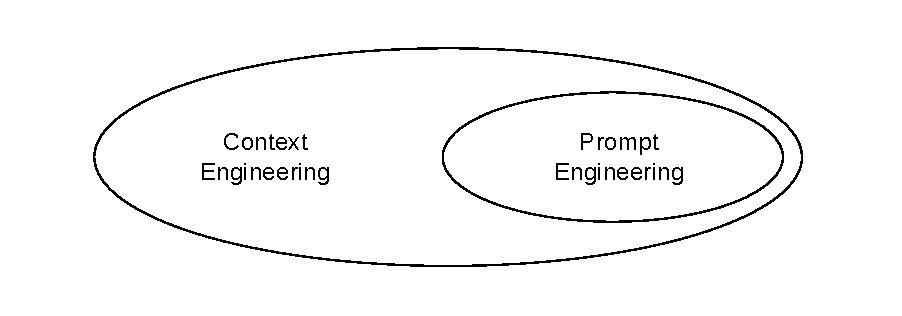
\includegraphics[width=0.9\textwidth]{assets/figures/02/venn-context-and-prompt-engineering.pdf}
  \caption{Venn-Diagram: Prompt Engineering as a subset of Context Engineering
  \figsource{Own illustration, created with draw.io.}}
  \label{fig:venn-diagram-prompt-engineering-context-engineering}
\end{figure}

Although various methods of context engineering are discussed in the literature, Mei et al.
critically point out that current practice operates without a unified theoretical foundation. Such a
foundation would be necessary to link the various techniques together and
derive principle-based design guidelines. This research gap is further exacerbated by the lack of
mathematical frameworks that would make it possible to characterize optimal design principles for context
engineering in complex systems. This is related to the lack of methods
for determining the optimal context composition. \cite[p. 51]{meiSurveyContextEngineering2025}

%%%%%%%
% ---------------------------------------------------------------------------------------------------------------------
\FloatBarrier
\subsection{Building blocks for LLM-based Workflows and Agents}
\label{sec:ai-agent-building-blocks}

In order to develop the AI agent described later, it was first necessary to examine the fundamental building
blocks of AI agents.
Anthropic has published a blog post on this topic, \cite{anthropicBuildingEffectiveAI}, which summarizes
these fundamental building blocks from their perspective and serves as the primary basis for this chapter. We
first examined all currently common patterns, even though not all of them were ultimately used in the actual system.

\newpage

\textbf{Prompt chaining}

\begin{figure}[H]
  \centering
  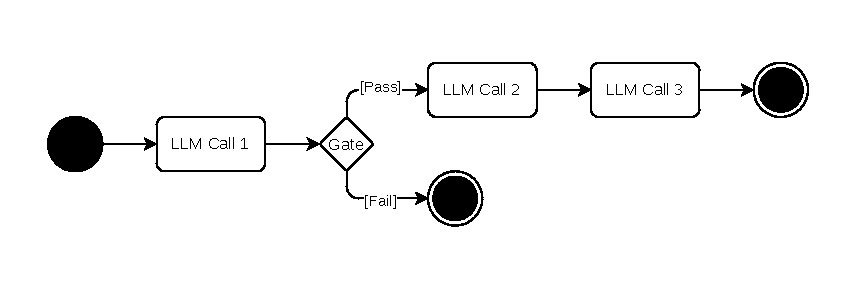
\includegraphics[width=0.9\textwidth]{assets/figures/02/prompt-chaining.pdf}
  \caption{AI-Building-Block:Prompt chaining: A complex task is decomposed into sequential LLM calls
    \figsource{Own illustration based on "Building Effective AI Agents by
  Anthropic"\cite{anthropicBuildingEffectiveAI}, created with draw.io.}}
  \label{fig:prompt-chaining}
\end{figure}

In prompt chaining, a complex task is broken down into a sequential series of substeps. Each step is
described by a prompt and an LLM call, which uses the result of the previous step as context for the next step.
Programmatic checks can be inserted in between. \cite{anthropicBuildingEffectiveAI}

\textbf{Routing}

\begin{figure}[H]
  \centering
  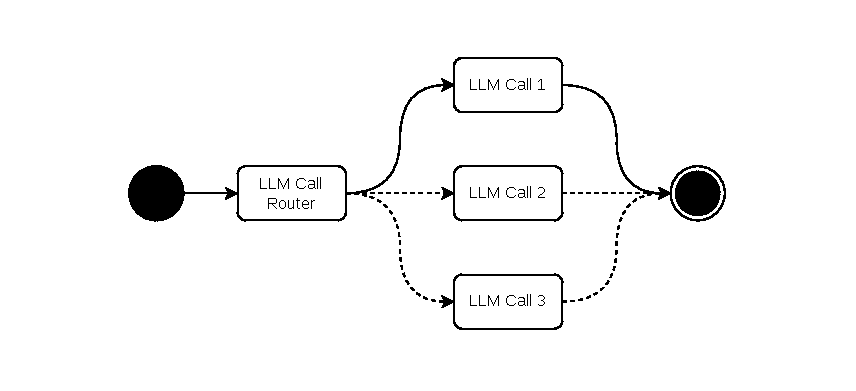
\includegraphics[width=0.9\textwidth]{assets/figures/02/routing.pdf}
  \caption{AI-Building-Block:Routing: A complex task is decomposed into subtasks and routed to specialized systems
    \figsource{Own illustration based on "Building Effective AI Agents by
  Anthropic"\cite{anthropicBuildingEffectiveAI}, created with draw.io.}}
  \label{fig:routing}
\end{figure}

During routing, tasks are classified and forwarded to subsystems that specialize in solving that category of
tasks. This results in a clear separation of responsibilities, which
is particularly well-suited when complex tasks can be divided into clearly definable categories and
processed by specialized LLMs, other AI models, or algorithms. \cite{anthropicBuildingEffectiveAI}

\textbf{Parallelization}

\begin{figure}[H]
  \centering
  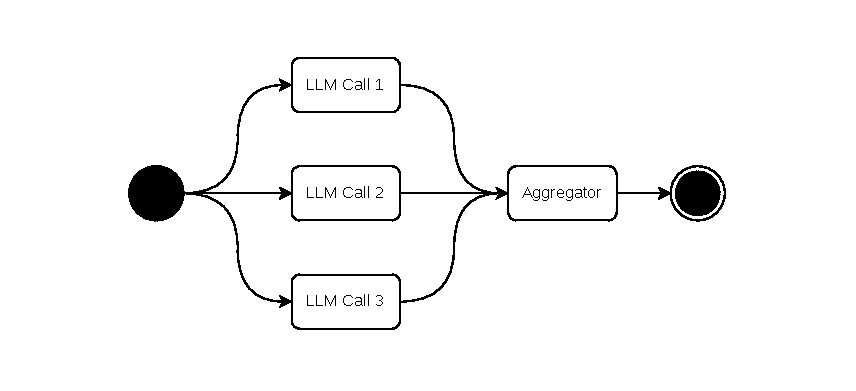
\includegraphics[width=0.9\textwidth]{assets/figures/02/parallelization.pdf}
  \caption{AI-Building-Block: Parallelization: Multiple tasks are processed in parallel and the results are
    aggregated programatically
    \figsource{Own illustration based on "Building Effective AI Agents by
  Anthropic"\cite{anthropicBuildingEffectiveAI}, created with draw.io.}}
  \label{fig:parallelization}
\end{figure}

In the parallelization workflow, multiple tasks are processed simultaneously, and the results
are aggregated programmatically. Typical use cases arise when tasks can be broken down into independent subtasks
or when multiple perspectives are required to achieve a more reliable result
(e.g. voting). For complex tasks with multiple aspects, LLMs achieve better results
when each aspect is addressed separately using a specialized prompt. \cite{anthropicBuildingEffectiveAI}

\textbf{Orchestrator-workers}

\begin{figure}[H]
  \centering
  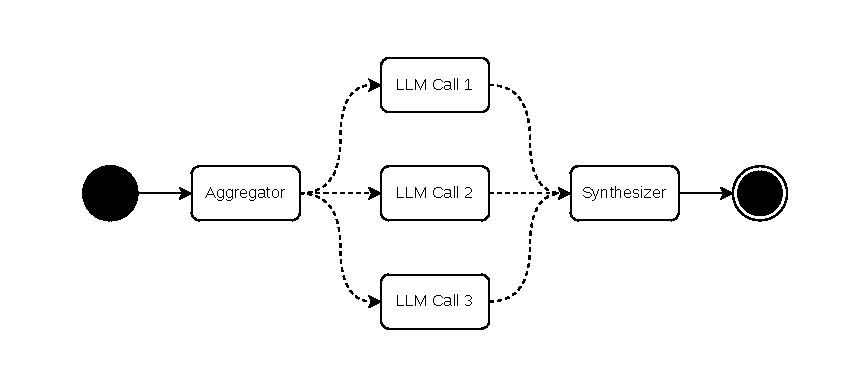
\includegraphics[width=0.9\textwidth]{assets/figures/02/orchestrator-workers.pdf}
  \caption{AI-Building-Block: Orchestrator-workers: A central LLM decomposes a main task dynamically into
    subtasks and delegates
    them to a variable number of worker LLMs
    \figsource{Own illustration based on "Building Effective AI Agents by
  Anthropic"\cite{anthropicBuildingEffectiveAI}, created with draw.io.}}
  \label{fig:orchestrator-workers}
\end{figure}

The Orchestrator-Worker workflow is similar to the parallelization workflow, but differs in that
it is used when the required subtasks are not known in advance. A central LLM dynamically breaks down
the main task into subtasks and delegates them to any number of worker LLMs,
whose results are then aggregated. \cite{anthropicBuildingEffectiveAI}

\textbf{Evaluator-optimizer}

\begin{figure}[H]
  \centering
  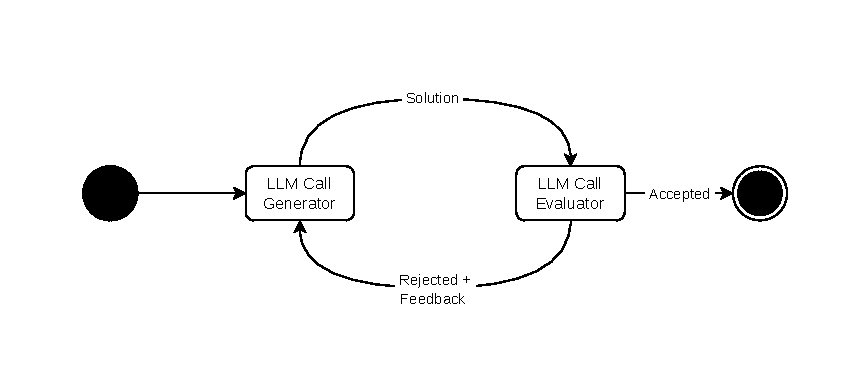
\includegraphics[width=0.9\textwidth]{assets/figures/02/evaluator-optimizer.pdf}
  \caption{AI-Building-Block: Evaluator-optimizer: A LLM generates answers, while another evaluates and
    optimizes them through feedback
    \figsource{Own illustration based on "Building Effective AI Agents by
  Anthropic"\cite{anthropicBuildingEffectiveAI}, created with draw.io.}}
  \label{fig:evaluator-optimizer}
\end{figure}

The evaluator-optimizer workflow uses a feedback loop in which one LLM generates responses while another
evaluates them and attempts to optimize them through feedback. This approach is particularly effective when
clear evaluation criteria are in place and iterative improvements are measurable. \cite{anthropicBuildingEffectiveAI}

% ---------------------------------------------------------------------------------------------------------------------
\subsection{Evaluating and Testing of AI-Systems}
\label{sec:evaluating-ai-systems}

Due to the probabilistic nature of AI-based systems, testing
AI-based systems differs fundamentally from conventional testing methods.

The International Software Testing Qualifications Board (ISTQB®) therefore suggests that this probabilistic
nature would require statistical testing methods. \cite[p. 39]{istqbrISTQBCertifiedTester}

An additional challenge is that some AI systems are not only static but also
adaptive, and can therefore continuously adjust themselves \cite[p.~39]{istqbrISTQBCertifiedTester}.

These adjustments can occur on at least two levels::
\begin{itemize}
  \item \textbf{Context-Based Adaptation:} Within the application, the AI system can dynamically adapt to
    changing conditions or the diverse possibilities offered by the
    context available at that moment.
  \item \textbf{Model-Based Adaptation:} Regardless of the specific context of the use case, the
    underlying AI models may change on their own, for example through the use of self-learning algorithms. When
    integrating external large language models (LLMs), the provider may make modifications to the model
    that are not immediately apparent to the user.
\end{itemize}
Defining a test oracle that is, specifying the expected outputs for specific input values for the system
under test is therefore extremely difficult or even impossible in complex AI systems
\cite[p.~39]{istqbrISTQBCertifiedTester}.

In a live meeting scenario, context-based adaptation is particularly relevant. In any given meeting, there
may be a variety of participants working on different topics, which makes the context in which the AI system
operates highly variable.

Mohammadi et al. \cite[p. 1]{mohammadiEvaluationBenchmarkingLLM2025} also point out that evaluating and
testing LLM-based agents is a complex and still under-researched field, particularly because
agents often operate in a more dynamic and interactive context.
They therefore describe the testing of LLM agents as an interplay of the various perspectives of natural
language processing (NLP), human-computer interaction (HCI), and software engineering.

\phantomsection\label{sec:code-based-testing}
Code-based methods aim to evaluate the performance of AI systems using explicit
program code, defined rules, and test cases with assertions. This involves verifying whether the
actions performed exactly meet specified criteria. \cite[p. 7]{mohammadiEvaluationBenchmarkingLLM2025}

For this purpose, for example, possible states that the system goes through can be modeled and analyzed using
trajectory comparisons. However, existing benchmarking methods such as AgentBoard
\cite{maAgentBoardAnalyticalEvaluation2024} are often
general in nature and only partially suitable for domain-specific use cases.

Code-based methods reach their limits, particularly with open-ended or qualitative responses, as well as with
creative problems where correctness
can be evaluated subjectively
\cite[p.~7]{mohammadiEvaluationBenchmarkingLLM2025}.

\phantomsection\label{sec:llm-as-a-judge}
The “LLM-as-a-Judge” approach leverages the reasoning capabilities of LLMs to evaluate agents' responses based on
qualitative criteria. In this process, the responses are analyzed based on
the evaluation metrics specified in the instructions. \cite[p.~7]{mohammadiEvaluationBenchmarkingLLM2025}.

The authors Zheng et al. \cite[p. 4]{zhengJudgingLLMasaJudgeMTBench2023} propose three variants of the
LLM-as-a-Judge approach, which can be applied individually or in combination:
\begin{itemize}
  \item Pairwise Comparison: An LLM compares two answers to a question and decides which is better or whether
    there is a tie.
  \item Single Answer Grading: An LLM evaluates a single answer directly using a scale or a set of criteria.
  \item Reference-Guided Grading: An LLM evaluates an answer by comparing it to a given
    reference solution, e.g., for math problems.
\end{itemize}

The appendix to the paper “Judging LLM-as-a-Judge with MT-Bench and Chatbot Arena” contains the corresponding
prompts that can be used for the various variants of the LLM-as-a-Judge approach
\cite{zhengJudgingLLMasaJudgeMTBench2023}.

According to Mohammadi et al., however, human-in-the-loop evaluation is still considered the gold standard, in which
people (such as in user studies, expert audits, or through crowdworkers) annotate or
evaluate the outputs \cite[p.~7]{mohammadiEvaluationBenchmarkingLLM2025}. However, this approach is often
difficult to scale and involves significant effort and costs.

A widely used approach is Evaluation-Driven Development (EDD), in which AI-based systems and agents
are continuously evaluated during the development phase to detect deviations and identify new use cases
\cite[p.~6]{mohammadiEvaluationBenchmarkingLLM2025}.
